\documentclass[tikz, margin=6mm]{standalone}
\usepackage[dvipsnames]{xcolor}
\usepackage{tikz}
\usetikzlibrary{arrows.meta, calc}
\pgfdeclarelayer{background}
\pgfsetlayers{background,main}
\definecolor{sxTeal}{HTML}{005B5B}
\definecolor{sxPortPurple}{HTML}{7A1B78}
\definecolor{sxSignalOrange}{HTML}{E46C2A}
\definecolor{sxFeedRed}{HTML}{C51B2B}
\definecolor{sxPanelGray}{HTML}{E6E6E6}
\definecolor{sxSoftBlue}{HTML}{E9F2F7}

% Chapter 4 architecture palette
\definecolor{sxExec}{HTML}{405BA9}
\definecolor{sxOrch}{HTML}{3B9C6B}
\definecolor{sxCore}{HTML}{E75E73}
\definecolor{sxAdapter}{HTML}{8E63A8}
\definecolor{sxSwitch}{HTML}{B86B00}
\definecolor{sxNeutralFill}{HTML}{F2F2F2}
\definecolor{sxNeutralBox}{HTML}{E0E0E0}
\definecolor{sxFrameworkBorder}{HTML}{666666}

\usetikzlibrary{patterns}
\tikzset{>=latex}

\tikzset{
  sx/base/.style={
    x=1cm,
    y=1cm,
    >=Latex,
    font=\sffamily
  },
  sx/panel/.style={
    draw=black!85,
    densely dotted,
    line width=1.0pt,
    rounded corners=1pt,
    fill=sxPanelGray
  },
  sx/data panel/.style={
    draw=black!85,
    densely dotted,
    line width=1.0pt,
    rounded corners=1pt,
    fill=white
  },
  sx/panel title/.style={
    draw=sxTeal,
    fill=sxTeal,
    text=white,
    minimum height=0.48cm,
    font=\sffamily\bfseries\large,
    inner xsep=4pt
  },
  sx/component/.style={
    rectangle,
    draw=sxTeal,
    fill=sxTeal,
    text=white,
    minimum width=1.85cm,
    minimum height=1.25cm,
    rounded corners=2pt,
    font=\sffamily\bfseries\large
  },
  sx/port/.style={
    rectangle,
    draw=sxPortPurple,
    fill=sxPortPurple,
    text=white,
    minimum size=4.2mm,
    inner sep=0pt,
    font=\sffamily\bfseries\small
  },
  sx/connection/.style={
    -{Latex[length=2.6mm,width=2.0mm]},
    draw=sxSignalOrange,
    line width=1.05pt
  },
  sx/feedthrough/.style={
    -{Latex[length=2.3mm,width=1.8mm]},
    draw=sxFeedRed,
    densely dotted,
    line width=0.95pt
  },
  sx/legend box/.style={
    draw=black!40,
    fill=white,
    rounded corners=2pt,
    line width=0.6pt
  },
  sx/data text/.style={
    anchor=north west,
    align=left,
    font=\sffamily\small
  },
  sx/data heading/.style={
    font=\sffamily\bfseries\small
  },
  sx/ch4/framework/.style={
    fill=sxNeutralFill,
    draw=sxFrameworkBorder,
    dashed,
    line width=0.8pt,
    rounded corners=5pt
  },
  sx/ch4/layerbg/.style={
    rounded corners=3pt,
    inner sep=3pt,
    draw=none
  },
  sx/ch4/layer label/.style={
    draw=white,
    rounded corners=3pt,
    minimum width=2.75cm,
    minimum height=1.12cm,
    text=white,
    align=center,
    font=\sffamily\footnotesize\bfseries
  },
  sx/ch4/item/.style={
    draw=black!18,
    rounded corners=3pt,
    minimum width=2.75cm,
    minimum height=1.12cm,
    text=black!82,
    align=center,
    font=\sffamily\footnotesize
  },
  sx/ch4/external item/.style={
    draw=black!20,
    fill=sxNeutralBox,
    rounded corners=3pt,
    minimum width=3.35cm,
    minimum height=1.12cm,
    text=black!78,
    align=center,
    font=\sffamily\footnotesize
  },
  sx/ch4/neutral box/.style={
    draw=black!38,
    rounded corners=4pt,
    fill=sxNeutralFill,
    line width=0.7pt
  },
  sx/ch4/arrow/.style={
    line width=1.0pt,
    draw=black!58,
    -{Latex[length=2.6mm, width=1.9mm]}
  },
  sx/ch4/toolcall/.style={
    line width=0.9pt,
    draw=black!50,
    dashed,
    -{Latex[length=2.4mm, width=1.8mm]},
    shorten >=2pt
  }
}

\newcommand{\sxPanelTitle}[3]{%
  \node[sx/panel title, minimum width=#3] at #1 {#2};%
}

\newcommand{\sxComponent}[3]{%
  \node[sx/component] (#1) at #2 {#3};%
}

\newcommand{\sxPort}[3]{%
  \node[sx/port] (#1) at #2 {#3};%
}

\newcommand{\sxdataheading}[1]{%
  \textbf{#1}%
}


% ─── Coordinate layout (y in cm, origin top-left, downward = negative) ────────
%
%  Title:                   [0.00 .. 0.85]   h=0.85
%  Port Interface header:   [0.85 .. 1.35]   h=0.50
%  Port Interface content:  [1.35 .. 2.85]   h=1.50
%  Two-column area:         [2.85 .. 10.85]  h=8.00
%
%  Left column  [x=0..5.5]  — Lifecycle
%    Header:                [2.85 .. 3.43]   h=0.58
%    Phase 1 Construction:  center y=3.88
%    Phase 2 Configuration: center y=4.78
%    Phase 3 Initialization:center y=5.68
%    Phase 4 Sim-Loop label:center y=6.43
%      4.1 Set Inputs:      center y=7.13
%      4.2 Do Step:         center y=8.13
%      4.3 Read Outputs:    center y=9.13
%    Phase 5 Reset/Release: center y=10.40
%
%  Right column [x=5.5..13] — three stacked sections
%    State Handling  hdr:   [2.85 .. 3.35]   h=0.50
%    State Handling  cnt:   [3.35 .. 5.85]   h=2.50
%      Physical State:      [x=5.65..9.10]  (solid border, mandatory)
%      Rollback:            [x=9.40..12.80] (dashed border, optional)
%    Struct Metadata hdr:   [5.85 .. 6.35]   h=0.50
%    Struct Metadata cnt:   [6.35 .. 8.35]   h=2.00  (dashed, optional)
%    Hybrid Capab    hdr:   [8.35 .. 8.85]   h=0.50
%    Hybrid Capab    cnt:   [8.85 .. 10.85]  h=2.00  (dashed, optional)
%
%  Legend (outside box):    [11.15 .. 11.90]

\begin{document}
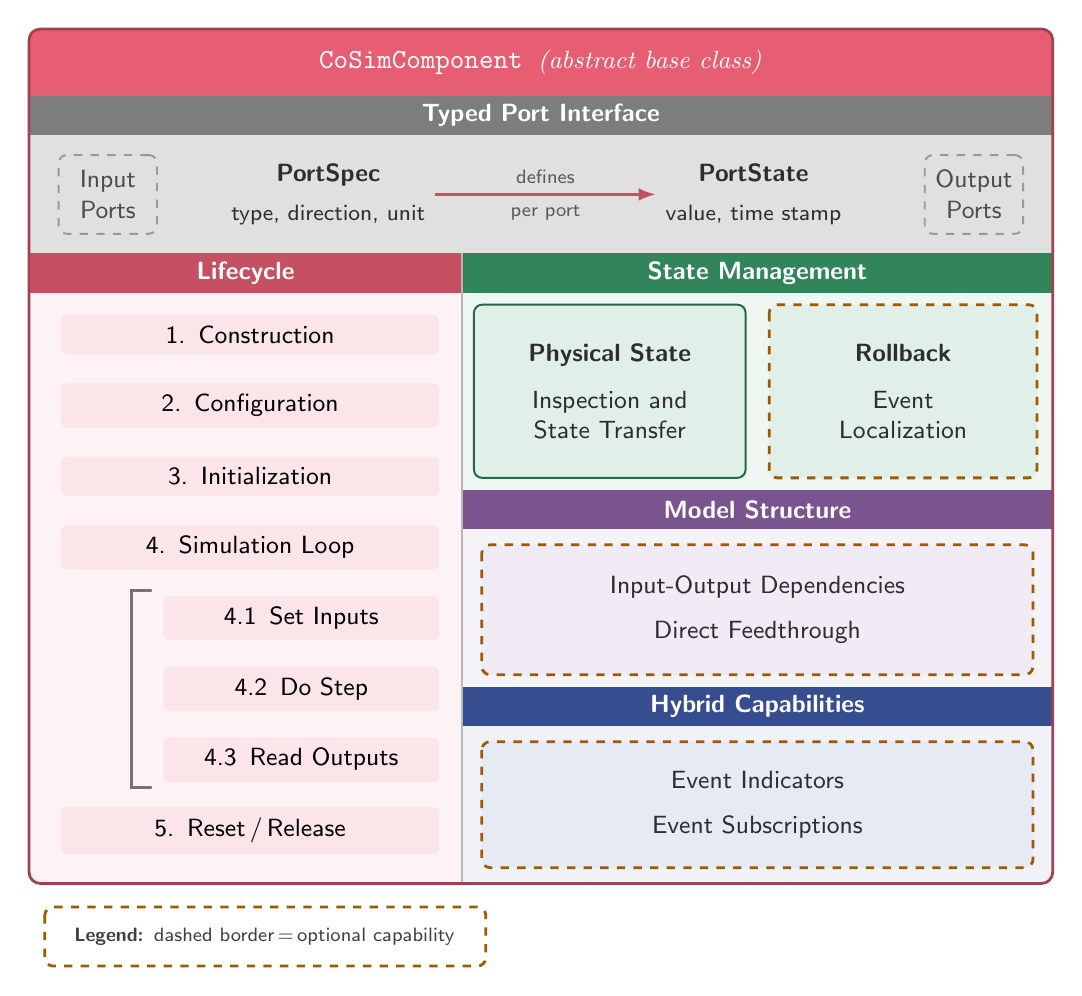
\begin{tikzpicture}[
  every node/.style = {font=\sffamily},
  % Arrow for PortSpec -> PortState
  arr/.style = {
    -{Latex[length=2.2mm, width=1.6mm]},
    draw=sxCore!85!black, line width=1.0pt,
  },
  % Dashed golden border: optional capability
  optbox/.style = {
    draw=sxSwitch!85!black, dashed, line width=1.0pt,
    rounded corners=3pt,
  },
  % Lifecycle step box (main phases)
  lifestep/.style = {
    fill=sxCore!16, rounded corners=2pt,
    inner xsep=8pt, inner ysep=4pt,
    minimum width=4.80cm,
    anchor=west, text=black, font=\sffamily\small,
  },
  % Lifecycle step box (indented simulation-loop sub-steps)
  simstep/.style = {
    fill=sxCore!16, rounded corners=2pt,
    inner xsep=8pt, inner ysep=4pt,
    minimum width=3.50cm,
    anchor=west, text=black, font=\sffamily\small,
  },
  % Dashed neutral border: port indicators
  portbox/.style = {
    draw=black!40, dashed, line width=0.7pt,
    rounded corners=3pt,
    minimum width=1.25cm, minimum height=1.0cm,
    align=center, text=black!70, font=\sffamily\small,
  },
]

% ============================================================================
% BACKGROUND FILLS
% ============================================================================
\begin{pgfonlayer}{background}

  \clip[rounded corners=4pt] (0,0) rectangle (13cm,-10.85cm);

  % ── Title ──────────────────────────────────────────────────────────────────
  \fill[sxCore] (0,0) rectangle (13cm,-0.85cm);

  % ── Port Interface ─────────────────────────────────────────────────────────
  \fill[sxFrameworkBorder!85] (0,-0.85cm) rectangle (13cm,-1.35cm);
  \fill[sxNeutralBox]         (0,-1.35cm) rectangle (13cm,-2.85cm);

  % ── Left: Lifecycle header + content ───────────────────────────────────────
  \fill[sxCore!85!black] (0,-2.85cm) rectangle (5.5cm,-3.35cm);
  \fill[sxCore!8]        (0,-3.35cm) rectangle (5.5cm,-10.85cm);

  % ── Right: State Handling ──────────────────────────────────────────────────
  \fill[sxOrch!85!black] (5.5cm,-2.85cm) rectangle (13cm,-3.35cm);
  \fill[sxOrch!8]        (5.5cm,-3.35cm) rectangle (13cm,-5.85cm);
  % Physical State sub-fill (slightly darker, mandatory sub-box)
  \fill[sxOrch!16] (5.65cm,-3.50cm) rectangle (9.10cm,-5.70cm);

  % ── Right: Structural Metadata ─────────────────────────────────────────────
  \fill[sxAdapter!85!black] (5.5cm,-5.85cm) rectangle (13cm,-6.35cm);
  \fill[sxAdapter!8]        (5.5cm,-6.35cm) rectangle (13cm,-8.35cm);

  % ── Right: Hybrid Capabilities ─────────────────────────────────────────────
  \fill[sxExec!85!black] (5.5cm,-8.35cm) rectangle (13cm,-8.85cm);
  \fill[sxExec!8]        (5.5cm,-8.85cm) rectangle (13cm,-10.85cm);

  % ── Column separator + outer border ────────────────────────────────────────
  \draw[black!28, line width=0.6pt] (5.5cm,-2.85cm) -- (5.5cm,-10.85cm);
\end{pgfonlayer}

\draw[sxCore!70!black, line width=1.0pt, rounded corners=4pt]
  (0,0) rectangle (13cm,-10.85cm);

% ============================================================================
% TITLE
% ============================================================================
\node[text=white, font=\sffamily\bfseries\normalsize, anchor=center]
  at (6.5cm,-0.425cm)
  {\texttt{CoSimComponent}%
   \enspace\normalfont\small\textit{(abstract base class)}};

% ============================================================================
% PORT INTERFACE
% ============================================================================
\node[text=white, font=\sffamily\bfseries\small, anchor=center]
  at (6.5cm,-1.10cm) {\textbf{Typed Port Interface}};

% Input Ports indicator
\node[portbox, anchor=center] at (1.00cm,-2.10cm) {Input\\Ports};

% PortSpec (named for arrow anchoring)
\node[text=black!82, align=center, anchor=center] (PSPEC) at (3.80cm,-2.10cm)
  {{\small\bfseries PortSpec}\\[2pt]{\footnotesize type,\ direction,\ unit}};

% PortState (named for arrow anchoring)
\node[text=black!82, align=center, anchor=center] (PSTATE) at (9.20cm,-2.10cm)
  {{\small\bfseries PortState}\\[2pt]{\footnotesize value,\ time stamp}};

% defines-per-port arrow
\draw[arr] (PSPEC.east) --
  node[above, font=\sffamily\scriptsize, text=black!65, pos=0.5] {defines}
  node[below, font=\sffamily\scriptsize, text=black!65, pos=0.5] {per port}
  (PSTATE.west);

% Output Ports indicator
\node[portbox, anchor=center] at (12.00cm,-2.10cm) {Output\\Ports};

% ============================================================================
% LIFECYCLE — header
% ============================================================================
\node[text=white, font=\sffamily\bfseries\small, anchor=center]
  at (2.75cm,-3.1cm) {\textbf{Lifecycle}};

% ============================================================================
% LIFECYCLE — numbered phases
% ============================================================================
% All items uniformly spaced at 0.90 cm center-to-center
\node[lifestep] at (0.40cm,-3.88cm) {1.\enspace Construction};

\node[lifestep] at (0.40cm,-4.78cm) {2.\enspace Configuration};

\node[lifestep] at (0.40cm,-5.68cm) {3.\enspace Initialization};

\node[lifestep] at (0.40cm,-6.58cm) {4.\enspace Simulation Loop};

% Bracket [ spanning sub-steps (top = 4.1 box top, bottom = 4.3 box bottom)
\draw[black!55, line width=0.9pt, line cap=round]
  (1.55cm,-7.13cm) -- (1.30cm,-7.13cm)
  -- (1.30cm,-9.63cm) -- (1.55cm,-9.63cm);

% Sub-step labels
\node[simstep] at (1.70cm,-7.48cm) {4.1\enspace Set Inputs};

\node[simstep] at (1.70cm,-8.38cm) {4.2\enspace Do Step};

\node[simstep] at (1.70cm,-9.28cm) {4.3\enspace Read Outputs};

\node[lifestep] at (0.40cm,-10.18cm) {5.\enspace Reset\,/\,Release};

% ============================================================================
% STATE HANDLING — header
% ============================================================================
\node[text=white, font=\sffamily\bfseries\small, anchor=center]
  at (9.25cm,-3.10cm) {\textbf{State Management}};

% ── Physical State sub-box (mandatory: solid border) ─────────────────────────
\draw[sxOrch!65!black, line width=0.7pt, rounded corners=3pt]
  (5.65cm,-3.50cm) rectangle (9.10cm,-5.70cm);

\node[text=black!82, font=\sffamily\small, align=center, anchor=center]
  at (7.375cm,-4.60cm)
  {{\small\bfseries Physical State}\\[6pt]
   Inspection and\\State Transfer};

% ── Rollback sub-box (optional: dashed golden border) ────────────────────────
\draw[optbox, fill=sxOrch!16] (9.40cm,-3.50cm) rectangle (12.80cm,-5.70cm);

\node[text=black!82, font=\sffamily\small, align=center, anchor=center]
  at (11.10cm,-4.60cm)
  {{\small\bfseries Rollback}\\[6pt]
   Event\\Localization};

% ============================================================================
% STRUCTURAL METADATA — header
% ============================================================================
\node[text=white, font=\sffamily\bfseries\small, anchor=center]
  at (9.25cm,-6.10cm) {\textbf{Model Structure}};

% ── Content (optional: dashed golden box) ────────────────────────────────────
\draw[optbox, fill=sxAdapter!13] (5.75cm,-6.55cm) rectangle (12.75cm,-8.20cm);

\node[text=black!82, font=\sffamily\small, align=center, anchor=center]
  at (9.25cm,-7.375cm)
  {Input-Output Dependencies\\[5pt]
   Direct Feedthrough};

% ============================================================================
% HYBRID CAPABILITIES — header
% ============================================================================
\node[text=white, font=\sffamily\bfseries\small, anchor=center]
  at (9.25cm,-8.60cm) {\textbf{Hybrid Capabilities}};

% ── Content (optional: dashed golden box) ────────────────────────────────────
\draw[optbox, fill=sxExec!13] (5.75cm,-9.05cm) rectangle (12.75cm,-10.65cm);

\node[text=black!82, font=\sffamily\small, align=center, anchor=center]
  at (9.25cm,-9.85cm)
  {Event Indicators\\[5pt]
   Event Subscriptions};

% ============================================================================
% LEGEND (below the figure, outside main box)
% ============================================================================
\draw[optbox] (0.20cm,-11.15cm) rectangle (5.80cm,-11.90cm);

\node[text=black!75, font=\sffamily\scriptsize, align=left, anchor=west]
  at (0.45cm,-11.525cm)
  {{\bfseries Legend:}\enspace dashed border\,=\,optional capability};

\end{tikzpicture}
\end{document}
